%----------------------------------------------------------------
%
%  File    :  vpn_prelim.tex
%
%  Author  :  Keith Andrews, IICM, TU Graz, Austria
% 
%  Created :  22 Feb 96
% 
%  Changed :  19 Feb 2004
% 
%----------------------------------------------------------------

\chapter{Preliminaries}

\label{chap:Preliminaries}

\section{Mealy Machines}
% TODO: Expand, add grafic or listing, see other papers for inspiration
Mealy machines are finite state machines where each output transition is defined by the current state and an input. More formally, a Mealy machine is defined as a 6-tuple $M = \{S, S_0, \Sigma, \Lambda, T, G\}$, where $S$ is a finite set of states, $S_0 \in S$ is the initial state, $\Sigma$ is a finite set called the input alphabet, $\Lambda$ is a finite set called the output alphabet, $T$ is the transition function $G: S \times \Sigma \rightarrow \Lambda$ which maps a state and an element of the input alphabet to another state in $S$ and $G$ is the output function $T: S \times \Sigma \rightarrow S$ which maps a state-input alphabet pair to an element of the output alphabet $\Lambda$. We use Mealy machines to model the state of learned IPsec implementations.

\section{Automata Learning}

% TODO: More on automata learning, in particular cover L* in detail. Consider what is repeated here from Related chapter.
Automata learning refers to methods of learning the state model, or automaton, of a system through an algorithm or process. We differentiate between active and passive automata learning. In passive automata learning (PAL), models are learned based on a given data set describing the behavior of the SUL, e.g. log files. In contrast, in active automata learning (AAL) the SUL is queried directly. In this paper, we will focus on AAL and will, moving on, be referring to it as automata learning or AAL interchangeably. 

AAL began in 1987 with a paper by Dana Angluin, titled ``Learning regular sets from queries and counterexamples''~\parencite{ANGLUIN198787}. In this seminal paper, Angluin introduced the $L^*$ algorithm, variants of which are still used for learning deterministic automata to this day, for example by the AAL python library \textsc{AALpy} \parencite{muvskardin2022aalpy}. While the original $L^*$ algorithm was designed to learn deterministic finite automata, the algorithm can be extended to learn Mealy machines \parencite{Niese2003AnIA}. While many modern implementations, including \textsc{AALpy} use improved versions of $L^*$, fundamentally they still resemble the original algorithm by Angluin. The base $L^*$ algorithm is briefly explained below.

% TODO: expand greatly, go into more detail here
$L^*$ works using a Minimally Adequate Teacher (MAT) model in which a learner queries a teacher about a SUL in order to learn the system. 

DEF TEACHER

DEF LEARNER

The teacher must be able to answer membership and equivalence queries posed by the learner regarding the SUL. 

Membership queries are used to check whether a word is included/accepted.

Equivalence queries are used to check if a learned model accurately matches the SUL. 

The learner, using the responses to its queries, then updates its model of the SUL. Learned models are commonly represented as Mealy machines. 





\section{Fuzzing}
% TODO: leave till we actually start this / could write the basics now --> show how model-based fuzzing can worl

\section{IPsec}
% TODO: More on VPNs in general

Virtual Private Networks (VPN) are used to extend and or connect private networks across an insecure channel (usually the public internet). They can be used e.g. to gain additional privacy from prying eyes such as Internet Server Providers, access to region-locked online content or secure remote access to company networks. Many different VPN protocols exit, including PPTP, OpenVPN and Wireguard. IPsec or IP Security, is a VPN layer 3 protocol used to securely communicate over an insecure channel. It is based on three sub-protocols, the Internet Key Exchange (IKE) protocol, the Authentication Header (AH) protocol and the Encapsulating Security Payload (ESP) protocol. IKE is mainly used to handle authentication and to securely exchange as well as manage keys. Following a successful IKE round, either AH or ESP is used to send packets securely between parties. The main difference between AH and ESP is that AH only ensures the integrity and authenticity of messages while ESP also ensures their confidentiality through encryption.

\begin{figure}[H]
\begin{centering}
	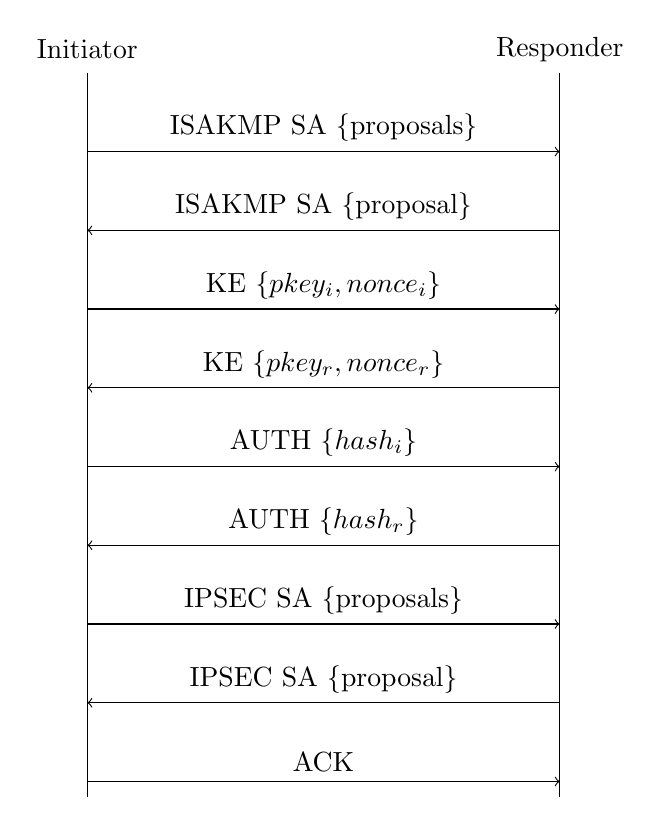
\begin{tikzpicture}[scale=1]
		\draw (-3,0) -- (-3,-9.2) (3,0) -- (3,-9.2);
		\node at (-3,.3) {Initiator};
		\node at (3,.3) {Responder};
		\draw[->] (-3,-1) -- node[midway,above] {ISAKMP SA \{proposals\}} (3,-1);
		\draw[<-] (-3,-2) -- node[midway,above] {ISAKMP SA \{proposal\}} (3,-2);
		\draw[->] (-3,-3) -- node[midway,above] {KE $\{pkey_i, nonce_i\}$} (3,-3);
		\draw[<-] (-3,-4) -- node[midway,above] {KE $\{pkey_r, nonce_r\}$} (3,-4);
		\draw[->] (-3,-5) -- node[midway,above] {AUTH $\{hash_i\}$} (3,-5);
		\draw[<-] (-3,-6) -- node[midway,above] {AUTH $\{hash_r\}$} (3,-6);
		\draw[->] (-3,-7) -- node[midway,above] {IPSEC SA \{proposals\}} (3,-7);
		\draw[<-] (-3,-8) -- node[midway,above] {IPSEC SA \{proposal\}} (3,-8);
		\draw[->] (-3,-9) -- node[midway,above] {ACK} (3,-9);
	\end{tikzpicture}
	\caption{IKEv1 between two parties}
	\label{fig:IKEv1}
\end{centering}
\end{figure}

The IKEv1 protocol works in two main phases, both relying on the Internet Security Association and Key Management Protocol (ISAKMP). Additionally, phase one can be configured to proceed in either Main Mode or Aggressive Mode. A typical exchange between two parties, an initiator and a responder, using Main Mode for phase 1, can be seen in Figure \ref{fig:IKEv1}. In phase one (Main Mode), the initiator begins by sending a Security Association (SA) to the responder. A SA essentially details important security attributes required for a connection such as the encryption algorithm and key-size to use, as well as the authentication method and the used hashing algorithm. These options are bundled in containers called proposals, with each proposal describing a possible security configuration. While the initiator can send multiple proposals to give the responder more options to choose from, the responder must answer with only one proposal, provided both parties can agree upon one of the suggested proposals. This initial communication is denoted as \emph{ISAKMP SA} in Figure~\ref{fig:IKEv1}. Subsequently, the two parties perform a Diffie-Hellman key exchange, denoted as \emph{KE}, and send each other nonces used to generate a shared secret key \emph{SKEYID} as detailed in Listing~\ref{lst:keying}. PSK refers to the pre-shared key, Ni/Nr to the initiator/responder nonce and CKY-I/CKY-R to the initiator/responder identifier cookie. Note that IKEv1 allows using various different authentication modes aside from PSK, including public key encryption and digital signatures. \emph{SKEYID} is used as a seed key for all further session keys \emph{SKEYID\_d}, \emph{SKEYID\_a}, \emph{SKEYID\_e}, with $g^{xy}$ referring to the previously calculated shared Diffie-Hellman secret and prf to a pseudo-random function (in our case, HMAC). Following a successful key exchange, all further messages of phase one and two are encrypted using a key derived from \emph{SKEYID\_e} and \emph{SKEYID\_a} for authentication. Finally, in the last section of phase one \emph{AUTH}, both parties exchange and verify hashes to confirm the key generation was successful. Once verification succeeds, a secure channel is created and used for phase two communication. If phase one uses Aggressive Mode, then only three packets are needed to reach phase two. While quicker, the downside of Aggressive Mode is that the communication of the hashed authentication material happens without encryption. This means, that using short pre-shared keys in combination with Aggressive Mode is inherently insecure, as the unencrypted hashes are vulnerable to brute-force attacks provided a short key-size~\footnote{https://nvd.nist.gov/vuln/detail/CVE-2018-5389}. The shorter phase two (Quick Mode) begins with another SA exchange, labeled with \emph{IPSEC SA} in Figure~\ref{fig:IKEv1}. This time, however, the SA describes the security parameters of the ensuing ESP/AH communication and the data is sent authenticated and encrypted using the cryptographic material calculated in phase one. This is followed by a single acknowledge message, \emph{ACK}, from the initiator to confirm the agreed upon proposal. After the acknowledgment, all further communication is done via ESP/AH packets, using \emph{SKEYID\_d} as keying material.

\begin{lstlisting}[float=ht, caption=IKE Keying, label=lst:keying]
	# For pre-shared keys: 
	SKEYID = prf(PSK, Ni_b | Nr_b)
	
	# to encrypt non-ISAKMP messages (ESP)
	SKEYID_d = prf(SKEYID, g^xy | CKY-I | CKY-R | 0)
	
	# to authenticate ISAKMP messages
	SKEYID_a = prf(SKEYID, SKEYID_d | g^xy | CKY-I | CKY-R | 1)
	
	# for further encryption of ISAKMP messages in phase 2
	SKEYID_e = prf(SKEYID, SKEYID_a | g^xy | CKY-I | CKY-R | 2)
\end{lstlisting}

In addition to the packets shown in Figure~\ref{fig:IKEv1}, IKEv1 also specifies and uses so called ISAKMP Informational Exchanges. Informational exchanges in IKEv1 are used to send ISAKMP Notify or ISAKMP Delete payloads. Following the key exchange in phase one, all Informational Exchanges are sent encrypted and authenticated. Prior, they are sent in plain. ISAKMP Notify payloads are used to transmit various error and success codes, as well as for keep-alive messages. ISAKMP Delete is used to inform the other communication partner, that a SA has been deleted locally and request that they do the same, effectively closing a connection. 

Compared to other protocols, IPsec offers a high degree of customizability, allowing it to be fitted for many use cases. However, in a cryptographic evaluation of the protocol, Ferguson and Schneier \textcite{ferguson1999cryptographic} criticize the complexity arising from the high degree of customizability as the biggest weakness of IPsec. To address its main criticism, IPsec-IKEv2 was introduced in RFC 7296 to replace IKEv1 \parencite{kaufman2014internet}. Nevertheless, IPsec-IKEv1 is still in wide-spread use to this day, with the largest router producer in Germany, AVM, still only supporting IKEv1 in their routers \parencite{avm2022}. We use IPsec-IKEv1 with Main Mode and ESP in this paper and focus on the IKE protocol as it is the most interesting from an AAL and security standpoint. % this part could maybe be moved to the introduction, not sure
